\documentclass[11pt]{article}

% Packages this paper needs
\usepackage{fullpage, hyperref,bbm,amssymb,amsfonts,amsthm}
\usepackage[noend]{algorithmic}
\usepackage{algorithm}
\usepackage{setspace}
\usepackage{cleveref}
\usepackage{color}
\usepackage{latexsym}
\usepackage{verbatim}
\usepackage{graphics}
\usepackage{graphicx}
\usepackage{multicol}



\newcommand{\<}{\langle}
\renewcommand{\>}{\rangle}
\newcommand{\C}{\mathbb{C}}
\newcommand{\cA}{\mathcal{A}}
\newcommand{\cB}{\mathcal{B}}
\newcommand{\cE}{\mathcal{E}}
\newcommand{\cF}{\mathcal{F}}
\newcommand{\cH}{\mathcal{H}}
\newcommand{\cK}{\mathcal{K}}
\newcommand{\cM}{\mathcal{M}}
\newcommand{\cR}{\mathcal{R}}
\newcommand{\cU}{\mathcal{U}}
\newcommand{\cV}{\mathcal{V}}
\newcommand{\cZ}{\mathcal{Z}}
\newcommand{\E}{\mathrm{\mathbf{E}}}
\newcommand{\Var}{\mathrm{\mathbf{Var}}}
\newcommand{\EE}[1]{\E\left(#1\right)}
\newcommand{\VV}[1]{\Var\left(#1\right)}
\newcommand{\s}{\mathrm{span}}
\newcommand{\R}{\mathbb{R}}

\renewcommand{\sim}{\mathrm{sim}}
\renewcommand{\prec}{\mathrm{prec}}
\newcommand{\fail}{\mathrm{fail}}
\newcommand{\median}{\mathrm{median}}
\newcommand{\anc}{\mathrm{anc}}

\newcommand{\kets}[1]{| #1 \rangle}                 % small ket vector
\newcommand{\bras}[1]{\langle #1 |}                 % small bra vector
\newcommand{\braket}[2]{\langle #1 | #2 \rangle}         % <x|y>
\newcommand{\ii}{\mathbb{I}}
% the I with two vertical lines
\newcommand{\norms}[1]{\big\| #1\big\|}          % norm
\newcommand{\ep}{\epsilon}

% the I with two vertical lines
\newcommand{\twonorm}[1]{\left\| #1\right\|_2}        % norm
\newcommand{\inftynorm}[1]{\left\| #1\right\|_\infty}
\newtheorem{fact}{Fact}

% epsilon
\newcommand{\tr}{\mathrm{tr}}
%\newcommand{\qed}{\hfill $\square$}
\newtheorem{definition}{Definition}
\newtheorem{theorem}{Theorem}
\newtheorem{lemma}{Lemma}
\newtheorem{proposition}{Proposition}
\newtheorem{cor}{Corollary}
\newtheorem{remark}{Remark}
\newtheorem*{problem}{Problem}


% style
\theoremstyle{definition}
\begin{document}
\title{Problem Set 1 for CS 540/495}
 \author{Michaela Laden, Caleb Perry, Tucker Mogren}				
\maketitle
%%%%%%%%%
\begin{abstract}  %
%%%%%%%%%
This report will summarize how the generic algorithm, Simulated Annealing, can be used in order 
\end{abstract}

%%%%%%%%%%%%
\section{Introduction} 
There are many cases where simulated annealing would be a valid generic algorithm to use in order to solve a specific problem. An example problem that benefits from the use of simulated annealing is the Vehicle Routing Problem. This problem is very similar to the common "Traveling Salesman" problem and explores how Simulated Annealing can be used to find the minimum costs between a set of delivery routes, where the originating and terminating location is a central terminal. There are many different variations of the Vehicle Routing Problem. Some variations focus on the use of different vehicle applications (EX: deliveries, tours, etc). This is a widely studied problem and using Simulated Annealing in order to find the best result for this problem has proven to be successful. 

%
%%%%%%%%%%%%


%%%%%%%%%%%%%%%
\section{The Background} 
%%%%%%%%%%%%%%%
\begin{problem}
The Vehicle Routing Problem is a problem that asks what is the best route for a fleet of vehicles to take in order to deliver to a certain set of customers within a given time period.\\
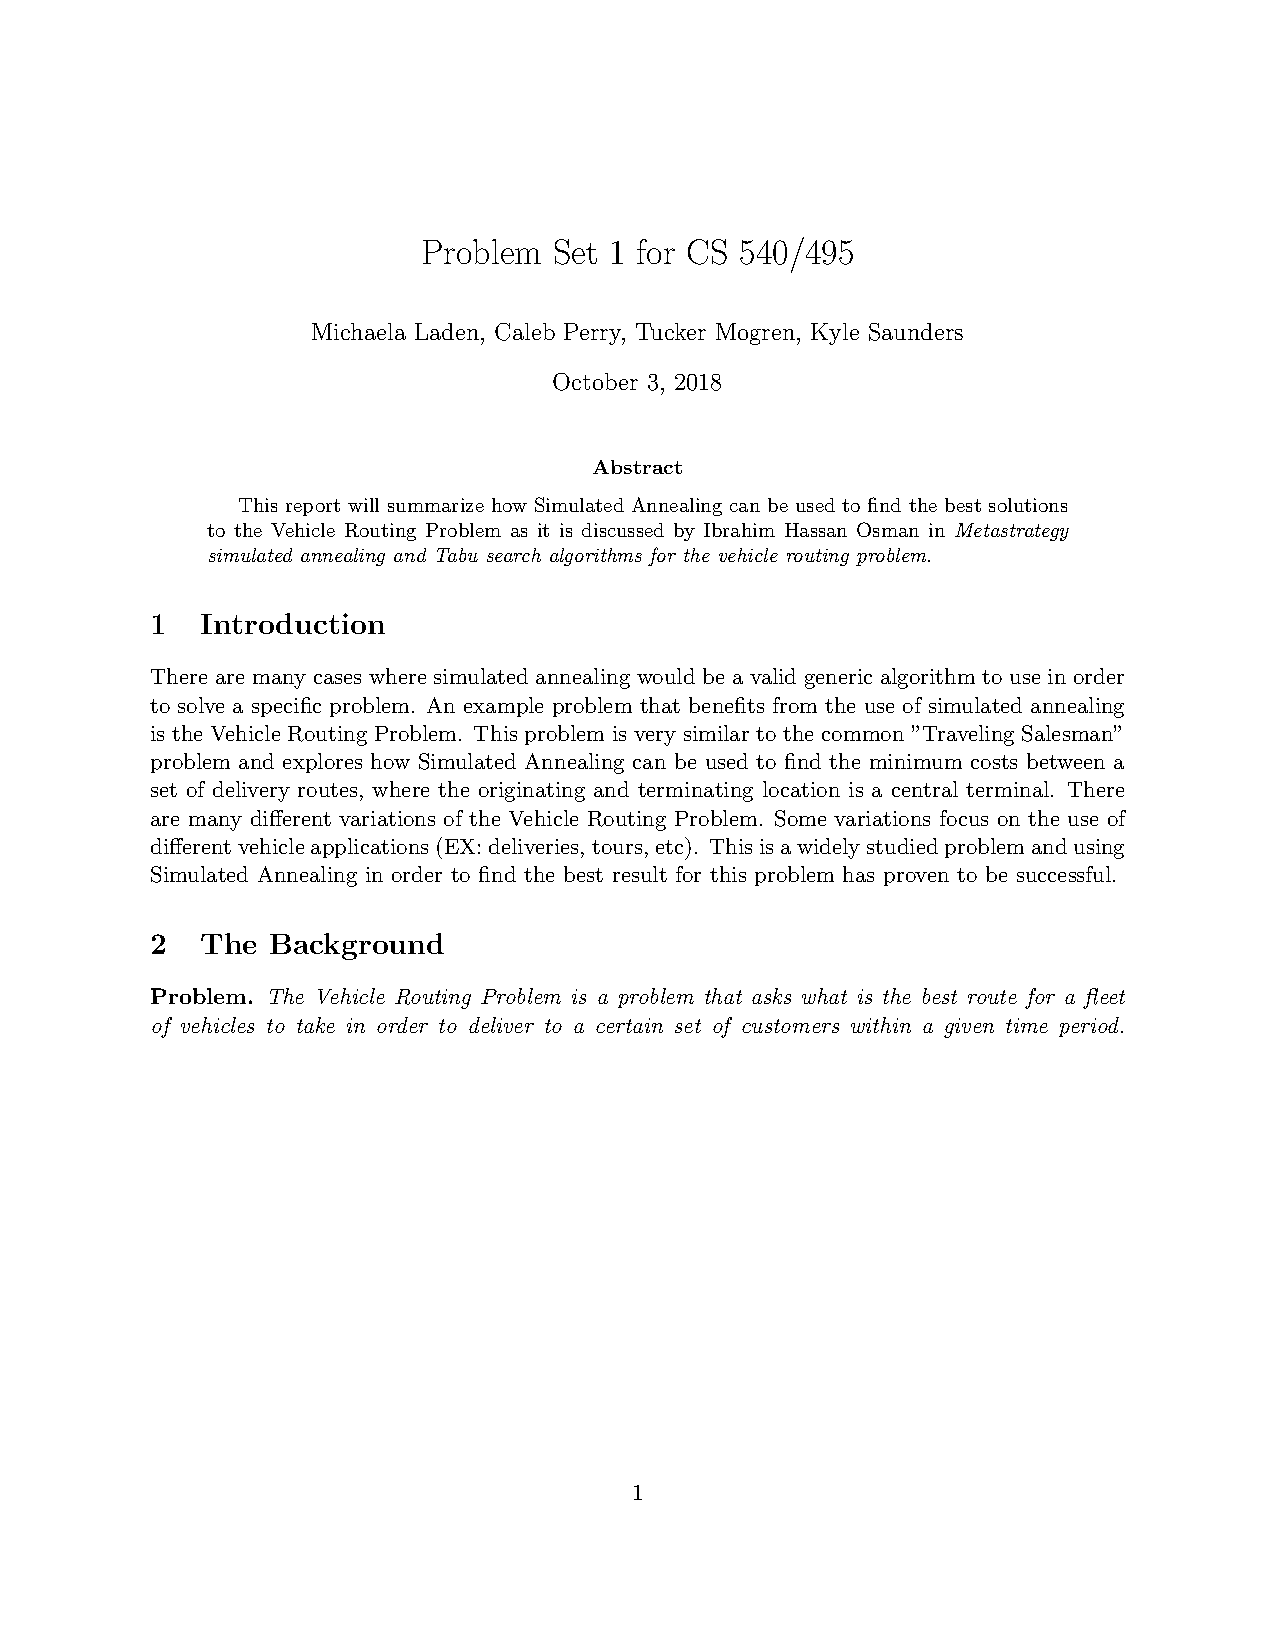
\includegraphics[width=\textwidth]{AI.PNG}\\
n = the number of customers\\
N = the set of Customers, N = \{1,..........n\}\\
$q_i$ = The demand of the customer i $\epsilon$ N (i = 0 denotes the depot, $q_0$ = 0)\\
$g_i$ = The service time of customer i $\epsilon$ N ($g_0$ = 0)\\
${c_i}_j$ = The travel time (distance) between customers i and j, ${c_i}_j$ = ${c_i}_j$ $\forall_i$, j $\epsilon$ N (${c_i}_j$ = $\infty$, $\forall$i $\epsilon$ N )\\
v = The number of vehicles, which is a \textit{decision} variable in our problem;\\
V = The set of vehicles, V = \{1,.......,v\};\\
Q = The vehicle capacity;\\
$R_p$ = The set of customers serviced by vehicle p;\\
C($R_p$) = The cost (length) of the optimal traveling salesmen tour $\pi_p$ over the customers in 
$R_p$$\cup$\{0\}. This cost includes the travel times (${c_i}_j$) and the service times ($\delta_i$);\\
L = The prespecified upper bound on the maximum tour length;\\
S = The feasible solution which is defined as S = \{$R_1$, ......, $R_v$\};\\
C(S) = The total sum of each individual tour length C($R_p$) for all P $\epsilon$ V\\\\\\
Our goal is to find the best solution  that minimizes the total travel length and time.
\end{problem}
\subsection{Diagrams}
\includegraphics[width=\textwidth]{AI2.PNG}\\
The above diagram shows two different kinds of routes the driver could take. Tour 1 shows a route where the driver starts at the Central terminal and makes all the proper stops, only returning to the terminal when the route is complete. The second tour, Tour 2, shows a route the driver would have to take if they had to return to the terminal number times during the route in order to restock packages.\\
\includegraphics[width=\textwidth]{AI3.PNG}\\
%%%%%%%%%%

\section{The Algorithm}
For the Vehicle Routing Problem (VPR) the specific algorithm used is the non-monotonic Simulated Annealing cooling schedule. This cooling schedule requires specifications such as, starting and final temperatures, decrement rule for updating the temperature $T_k$ after each iteration k, update rule for temperature reset variables Tr after the system freezes, stopping criterion R, which is the total number of temperature resets to be performed after the best solution was found. This method uses 1-interchange mechanism to generate neighbouring solutions where the neighborhoods are then searched in the indicated order. The algorithm performs a single iteration at each temperature.  

\subsection{The Procedure}
\\Describe how the algorithm is used  (for instance) ; and maybe how it differs from the regular implementation (any clever ideas, such as nice data structure designed for this problem for efficient storage purpose; or any interesting reduction
in the algorithm steps;.\\
\\\textbf{Step 1}: Generate an initial heuristic solution S by the savings method.\\
\\\textbf{Step 2}: Initialize the cooling schedule parameters: 
perform a test cycle of search over the neighborhood \textit{N(S)} of the initial solution without performing the exchanges in order to obtain the largest and smallest $\Delta_{max}$ change in objective function values, and an estimate of the total number of feasible exchanges \textit{Nfeas}.
Set {$T_s$=$\Delta_{max}$, $T_f$=$\Delta_{min}$, $T_r=T_s$, $\alpha$ = n\times Nfeas, $\gamma$ = n, R=3, $s_b$=S and k=1}\\
\\\textbf{Step 3}: Select a solution S'\in$N_1$(S) in ordered search and compute $\Delta$ = \textit{C(S')-C(S)} according to cost evaluation procedure.\\
\\\textbf{Step 4}: If {($\Delta \leq 0$ or $\Delta > 0$ and e$^{-\Delta/T_k}$ $\geq \theta$, where $\theta$ is a uniform random parameter 0 $< \theta <1$}
\textbf{Then} accept the new solution \textit{S'}, compute $\Delta$ according to cost procedure(b), set \textit{S=S'}
    if \textit{$C(S')<C(S_b)$}, then \textit{$S_b=S'$} and \textit{$T_b = T_k$}, the temperature at which the best solution is found;
    \textbf{otherwise} return \textit{S}.\\
\\\textbf{Step 5}: Update temperatures according to:\\ 
\\\textit{Normal decrement rule:}\\
\\$T_{k}$=$\frac{T_{k}}{1+\beta_{k}T_{k}}$, where $\beta_{k}$=$\frac{T_{s}-T_{f}}{(\alpha + \gamma \sqrt{k}) T_{s}T_{f}}$;\\
\\or \textit{Occasional increment rule:} If a cycle of search is comleted without accepting any 1-interchange move, update as\\
\\ $T_{r}$= $max $

%%%%%%%%%%%%%%%%%%%%%%%%%%%%%%%%%%%%%%%%%%%%%%%%%%%%%%%%%%%%%%%%%%%%%%
\section{The Complexity \& Discussion}
%%%%%%%%%%%%%%%%%%%%%%%%%%%%%%%%%%%%%%%%%%%%%%%%%%%%%%%%%%%%%%%%%%%%%%
The gain in complexity, theoretically or heuristically such as where it excels. Furthermore, can you describe where this can be further \textbf{improved} or any related work that can be benefit from this line of research? 


As stated above, this problem very closes mirrors the Traveling Salesman problem and its solution can be directly implemented when derived from the Traveling Salesman. A situation like this requires thousands, if not millions of iterations in order to find the best, most efficient solution. 


The Vehicle Routing Problem, takes into account capacity, and distance restrictions that are involved in the process of designing and discovering minimum delivery costs. It is understood that one vehicle will be assigned to one route and that the vehicle that is assigned to said route will not have its predetermined capacity exceeded. 

%%%%%%%%%%%%%%%%%%%%%%%%%%%%%%%%%%%%%%%%%%%%%%%%%%%%%%%%%%%%%%%%%%%%%%
\begin{thebibliography}{9}
\bibitem{Metastrategy simulated annealing and Tabu search
algorithms for the vehicle routing problem} 
Ibrahim Hassan Osman,
Metastrategy simulated annealing and Tabu search
algorithms for the vehicle routing problem.
\end{thebibliography}

\end{document}
%%%%%%%%%%%%%%%%%%%%%%%%%%%%%%%%%%%%%%%%%%%%%%%%%%%%%%%%%%%%%%%%%%%%%%%%%%%%%%%%%
